\chapter{Proof of Concept}
\label{ch:proof-of-concept}
Dit hoofdstuk bevat het vergelijkend experiment tussen twee eerder gekozen open source serverless (FaaS) frameworks, namelijk Fission en OpenFaaS. In dit onderdeel worden de twee frameworks opgezet op een Kubernetes cluster die bestaat uit één node. Beide frameworks worden opgezet op een MacBook Pro waarop Minikube draait. Minikube is een ''Out-of-the-box'' Kubernetes cluster die overal kan draaien. Er wordt gekozen om gebruik te maken van Minikube omdat op deze manier beide frameworks op identiek dezelfde hardware kunnen gedraaid worden. Daarnaast biedt Minikube dezelfde functionaliteiten als een volledige Kubernetes cluster die elders is opgezet. Dit hoofdstuk is opgedeeld in twee grote onderdelen waarbinnen telkens dezelfde secties met dezelfde stappen voor elk framework terug te vinden zijn. Daarnaast is er eveneens een sectie in dit hoofdstuk terug te vinden waarin de demo functie die serverless gedraaid zal worden op de frameworks wordt voorgesteld. De demo bestaat uit het deployen van een Python functie die de functionaliteit van beide frameworks demonstreert en de executietijd van de functie meet. Later wordt er in dit onderzoek een vergelijking tussen Fission en OpenFaaS gemaakt waarbij onder meer gekeken zal worden naar het verschil in executietijd tussen de geschreven functie alsook de gebruiksvriendelijkheid. Deze Proof of Concept moet meer inzicht geven in beide frameworks en geeft een duidelijk beeld van wat deze precies inhouden.
\\\\
\section{Voorbereiding omgeving}
\label{sec:voorbereiding-omgeving}
\subsection{Onderliggende hardware}
Het experiment zal worden uitgevoerd op een MacBook Pro, model 2018 met volgende specificaties:
\begin{itemize}
    \item Processor: 2,2 GHz Intel Core i7
    \item Memory: 16 GB 2400 MHz DDR4
    \item Graphics: Radeon Pro 555X 4 GB en Intel UHD Graphics 630 1536 MB
    \item Opslag: 256 GB SSD
\end{itemize}

\subsection{Homebrew}
Om de opstelling van het experiment klaar te zetten is het zinvol gebruik te maken van Homebrew\footnote{https://brew.sh/}, dit is een packetmanager ontwikkeld voor macOS. Homebrew zorgt ervoor dat softwarepakketten kunnen worden gedownload uit bestaande repositories. In de verdere uitwerking van dit onderzoek wordt Homebrew eveneens gebruikt voor het installeren van software.\\\\
Homebrew kan worden geïnstalleerd door volgend commando in de Terminal uit te voeren: 
\begin{lstlisting}[language=bash]
$ /usr/bin/ruby -e "$(curl -fsSL 
https://raw.githubusercontent.com/Homebrew/install/master/install)"
\end{lstlisting}

\subsection{Softwarepakketten}
Alvorens de frameworks kunnen worden opgezet moeten er reeds enkele softwarepakketten worden geïnstalleerd. Enerzijds is Docker nodig als container engine, anderzijds Kubernetes als container platform. Daarnaast is er ook een hypervisor nodig die het draaien van een Minikube cluster mogelijk maakt. In dit onderzoek wordt gebruik gemaakt van VirtualBox als hypervisor, deze is open source en gratis. De softwarepakketten kunnen als volgt succesvol geïnstalleerd worden met Homebrew:        
\begin{lstlisting}[language=bash]
$ brew tap caskroom/cask
$ brew cask install virtualbox
$ brew cask install docker
$ brew cask install minikube
$ brew install kubernetes-cli
\end{lstlisting}

\section{Python demofunctie}
Om de werking van beide frameworks te demonstreren wordt er gekozen voor een functie in Python. De functie wordt aangeroepen via de API van het framework waarop deze draait. De demofunctie is eenvoudig en bestaat uit een print statement dat de gebruiker verwelkomt, vervolgens wordt er een loop uitgevoerd die ervoor zorgt dat de functie toch even loopt en uiteindelijk wordt deze uitvoeringstijd weggeschreven naar een Google Spreadsheet bestand. De Python functie maakt gebruik van de Google API voor het wegschrijven naar het spreadsheet bestand. De functie wordt verpakt in een Docker image zodat deze kan worden gedeployed op beide frameworks zonder dat deze nog moet worden gebuild. De Docker image met de functie is gepubliceerd op de Docker Hub repository van Lennert Mertens. Om gebruik te kunnen maken van Google spreadsheets moet er een Google project worden aangemaakt via de Google API, deze stappen staan verder beschreven.

\subsection{Google API}
De Python functie schrijft de executietijd van de functies weg naar een bestand op Google spreadsheets. Om gebruik te maken van een spreadsheet bestand moet eerst de API worden geconfigureerd, daarnaast moeten ook de credentials op de demo machine worden geconfigureerd. Het Goolge project wordt opgezet zodat de functie data kan wegschrijven naar de spreadsheet

\subsection{Code}
\begin{lstlisting}[language=python]
# demofunctie.py
import time
start = time.time()
print("Hello everyone, this is a serverless demo function!")
a = range(1000000)
b = []
for i in a:
    b.append(i*2)
end = time.time()
execution_time= end - start
print(execution_time)
\end{lstlisting}

\subsection{Google spreadsheets}

\section{OpenFaaS}
Het eerste framework dat wordt uitgetest is OpenFaaS. Het experiment wordt opgezet op een MacBook Pro die voldoet aan voorgaande specificaties en beschikt over de benodigde softwarepakketten zoals eerder ook beschreven werd. De stappen die doorlopen worden in het opzetten en uitvoeren van het experiment, zijn steeds duidelijk gedocumenteerd en staan chronologisch gerangschikt. De installatieprocedure is eenvoudig te volgen en is reproduceerbaar aan de hand van de gedocumenteerde stappen en bijhorende scripts.
\\\\\\
\subsection{Configuratie Minikube}
Vooraleer OpenFaaS geïnstalleerd kan worden, wordt er een lokale Kubernetes cluster die bestaat uit één node opgezet met Minikube. Een Minikube cluster biedt dezelfde functionaliteiten als een productieomgeving waarop een Kubernetes cluster is geïnstalleerd. Er wordt gebruik gemaakt van Kubernetes als container orchestrator. Een orchestrator is een tool die instaat voor het management van containers en microservice applicaties. Kubernetes zorgt ervoor dat applicaties schaalbaar kunnen worden opgezet, staat in voor het volledige beheer van de containers en voorziet ''High-availability''.
\\
In sectie \ref{sec:voorbereiding-omgeving} werden de benodigde softwarepakketten reeds geïnstalleerd. Indien alle stappen succesvol werden doorlopen dan kan de Minikube cluster probleemloos als volgt worden gestart. Na de installatie wordt eerst ook de status van de cluster nagegaan.

\begin{lstlisting}[language=bash]
$ minikube start
$ minikube status
\end{lstlisting}

De uitvoer van het tweede commando geeft een overzicht dat er als volgt zou moeten uitzien, het IP adres wijkt mogelijks af van hetgene in de output. Wanneer de output overeenkomt met deze dan is Minikube succesvol geïnstalleerd.
\begin{lstlisting}[language=bash]
host: Running
kubelet: Running
apiserver: Running
kubectl: Correctly Configured: pointing to \ 
minikube-vm at 192.168.99.107
\end{lstlisting}

\subsection{Installatie OpenFaaS}
Indien de installatie van Minikube uit voorgaande sectie succesvol is, dan kan OpenFaaS worden geïnstalleerd. De installatie van OpenFaaS bestaat uit enkele stappen die werden omgevormd tot een shell script. Het is mogelijk dit script vanuit de Terminal uit te voeren, vervolgens start de installatie van OpenFaaS. De volledige installatie van het framework is geautomatiseerd en reproduceerbaar. Het script is terug te vinden als bijlage \ref{sec:installatie-openfaas} onder de naam Installatiescript OpenFaaS. De installatie is gebaseerd op een blogpost van \textcite{Ellis2017}, de founder van OpenFaaS. In de documentatie van OpenFaaS\footnote{https://docs.openfaas.com/} wordt eveneens naar deze blogpost gerefereerd als installatiehandleiding. Na de  uitvoering van het script is OpenFaaS geïnstalleerd bovenop de Minikube cluster. Na de installatie worden enkele artefacten geproduceerd die communicatie met het framework mogelijk maken.
\\
\begin{itemize}
    \item OpenFaaS UI standaard poort: 31112
    \item OpenFaaS UI URL: http://MINIKUBE-IP:31112/ui/
\end{itemize}
\subsection{Gebruik OpenFaaS}
\subsubsection{User Interface}
Na de installatie is het mogelijk naar de OpenFaaS UI te surfen, \\bijvoorbeeld: http://192.168.99.107:31112. 
De eerste keer dient er aangemeld te worden met gebruiker ''admin'' (Deze gebruiker wordt aangemaakt in het installatiescript) en het wachtwoord dat in de Terminal werd weergegeven door het installatiescript. Na het aanmelden is de interface zoals in figuur \ref{fig:openfaas-ui} te zien. De UI ziet er vrij sober uit na installatie, er is eveneens een mogelijkheid om een nieuwe functie te deployen via de ''Deploy New Function'' knop. Wanneer gebruikers kiezen een nieuwe functie te deployen dan kunnen ze enerzijds kiezen voor een community functie, dit zijn reeds bestaande functies die op het OpenFaaS framework gedraaid kunnen worden. Anderzijds kunnen gebruikers ook manueel zelfgeschreven functies deployen aan de hand van deze interface. In dit onderzoek worden functies gedeployed via de command-line aan de hand van het faas-cli commando. Deployments van functies via de command line biedt een betere reproduceerbaarheid en is vaak sneller en makkelijker te reproduceren. Er wordt ook bewust gekozen voor de command-line tools omdat niet alle serverless frameworks over een UI beschikken. De interface is een leuke feature en is makkelijk in gebruik voor mensen die aan de slag willen met serverless, deze wordt eveneens standaard meegeïnstalleerd met OpenFaaS.
\begin{figure}
    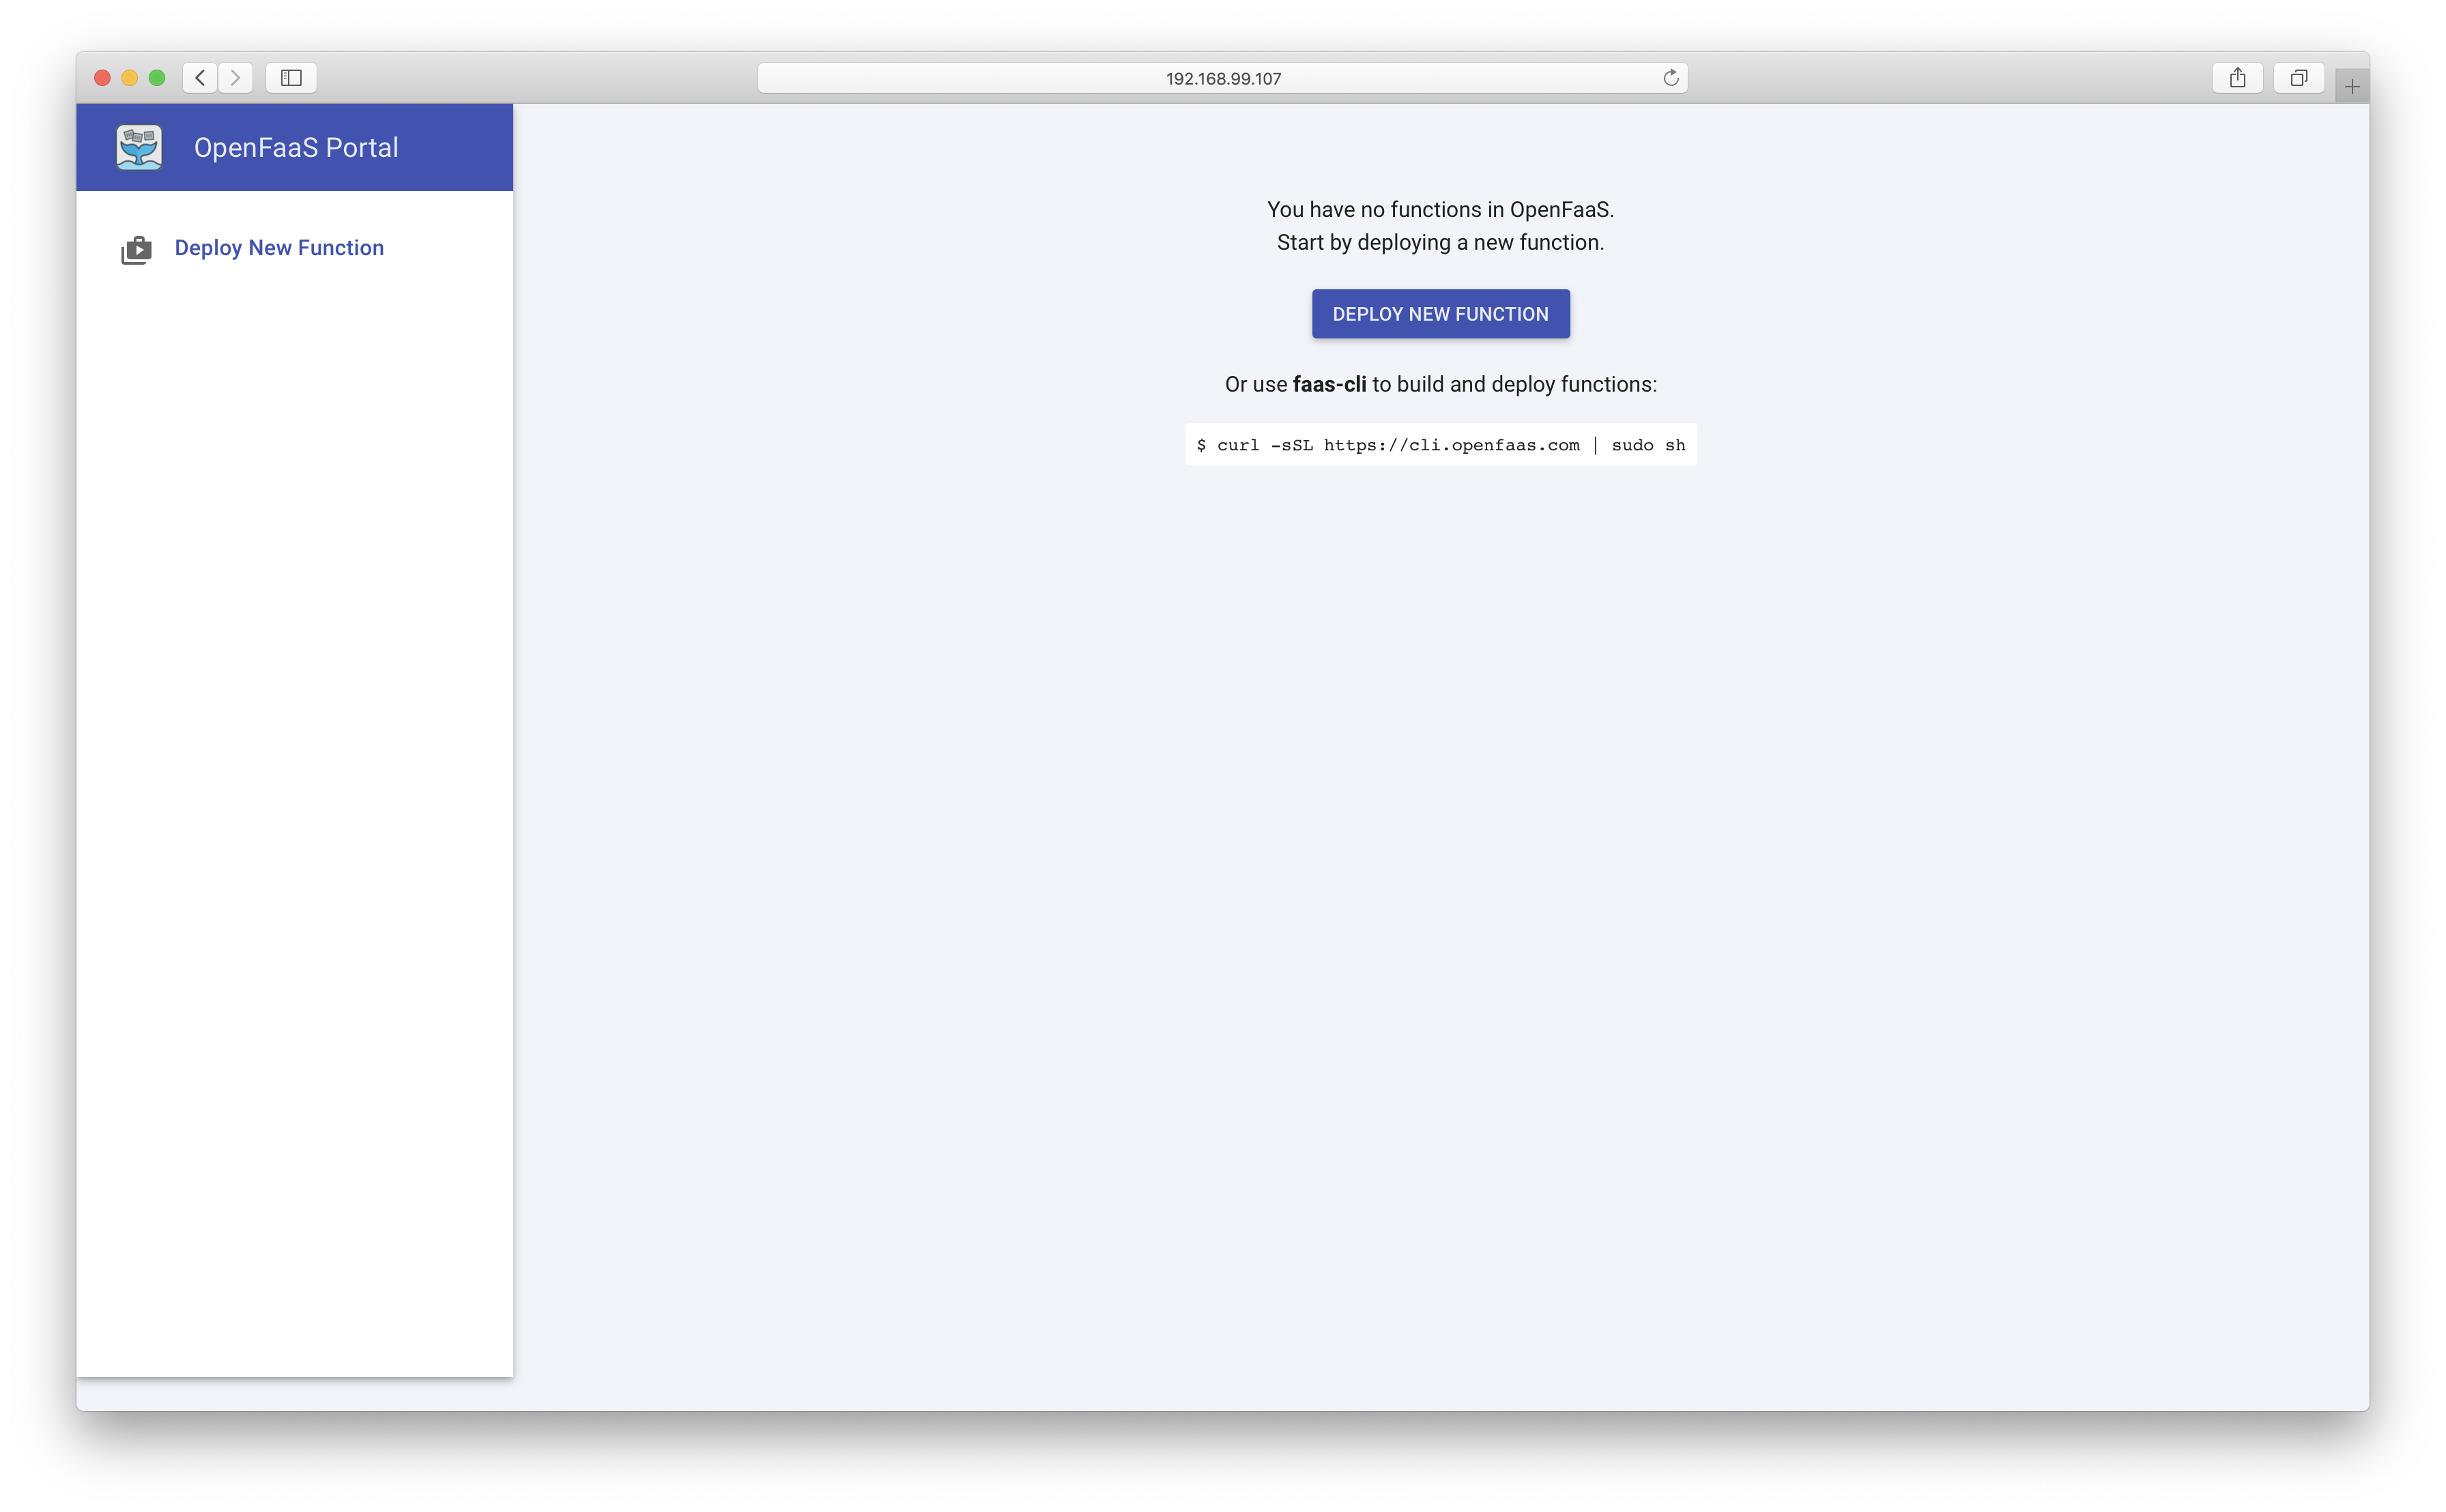
\includegraphics[width=1\textwidth]{img/openfaas-ui.png}
    \caption{OpenFaaS User Interface}
    \label{fig:openfaas-ui}  
\end{figure}

\subsubsection{Command-line tools}
Faas-cli is de command-line tool die beheer van OpenFaaS voorziet aan de hand van de console. Vooraleer van start te kunnen gaan moet de gebruiker inloggen via de Terminal door volgend commando in te voeren. Het paswoord is hetgene dat eerder in de Terminal werd weggeschreven, net zoals het IP adres waarop OpenFaaS draait.
\begin{lstlisting}[language=bash]
$ faas-cli login -g http://$OPENFAAS_URL -u admin -p $PASSWORD
\end{lstlisting}
De command-line tools voorzien dezelfde functionaliteiten als die van de UI. Het is mogelijk om functies te deployen via de CLI. Later in dit onderzoek zal de demofunctie die werd geschreven aan de hand van de command-line tools worden gedeployed.

\subsubsection{Prometheus monitoring}
OpenFaaS voorziet ook monitoring aan de hand van Prometheus, via een Grafana dashboard kunnen verschillende metrics van functies worden bekeken. De configuratie van het dashboard werd reeds voorzien in installatiescript \ref{sec:installatie-openfaas}. Na de configuratie van Prometheus en Grafana kan het dashboard worden geraadpleegd via de GRAFANA\_URL, bijvoorbeeld http://192.168.99.107:32548/dashboard/db/openfaas. In figuur \ref{fig:grafana-dashboard} is het Grafana dashboard zichtbaar dat wordt weergegeven bij het openen van de link. Alvorens dit scherm kan geraadpleegd worden dient de gebruiker in te loggen met de standaard gebruiker ''admin'' met wachtwoord ''admin''.
\begin{figure}
    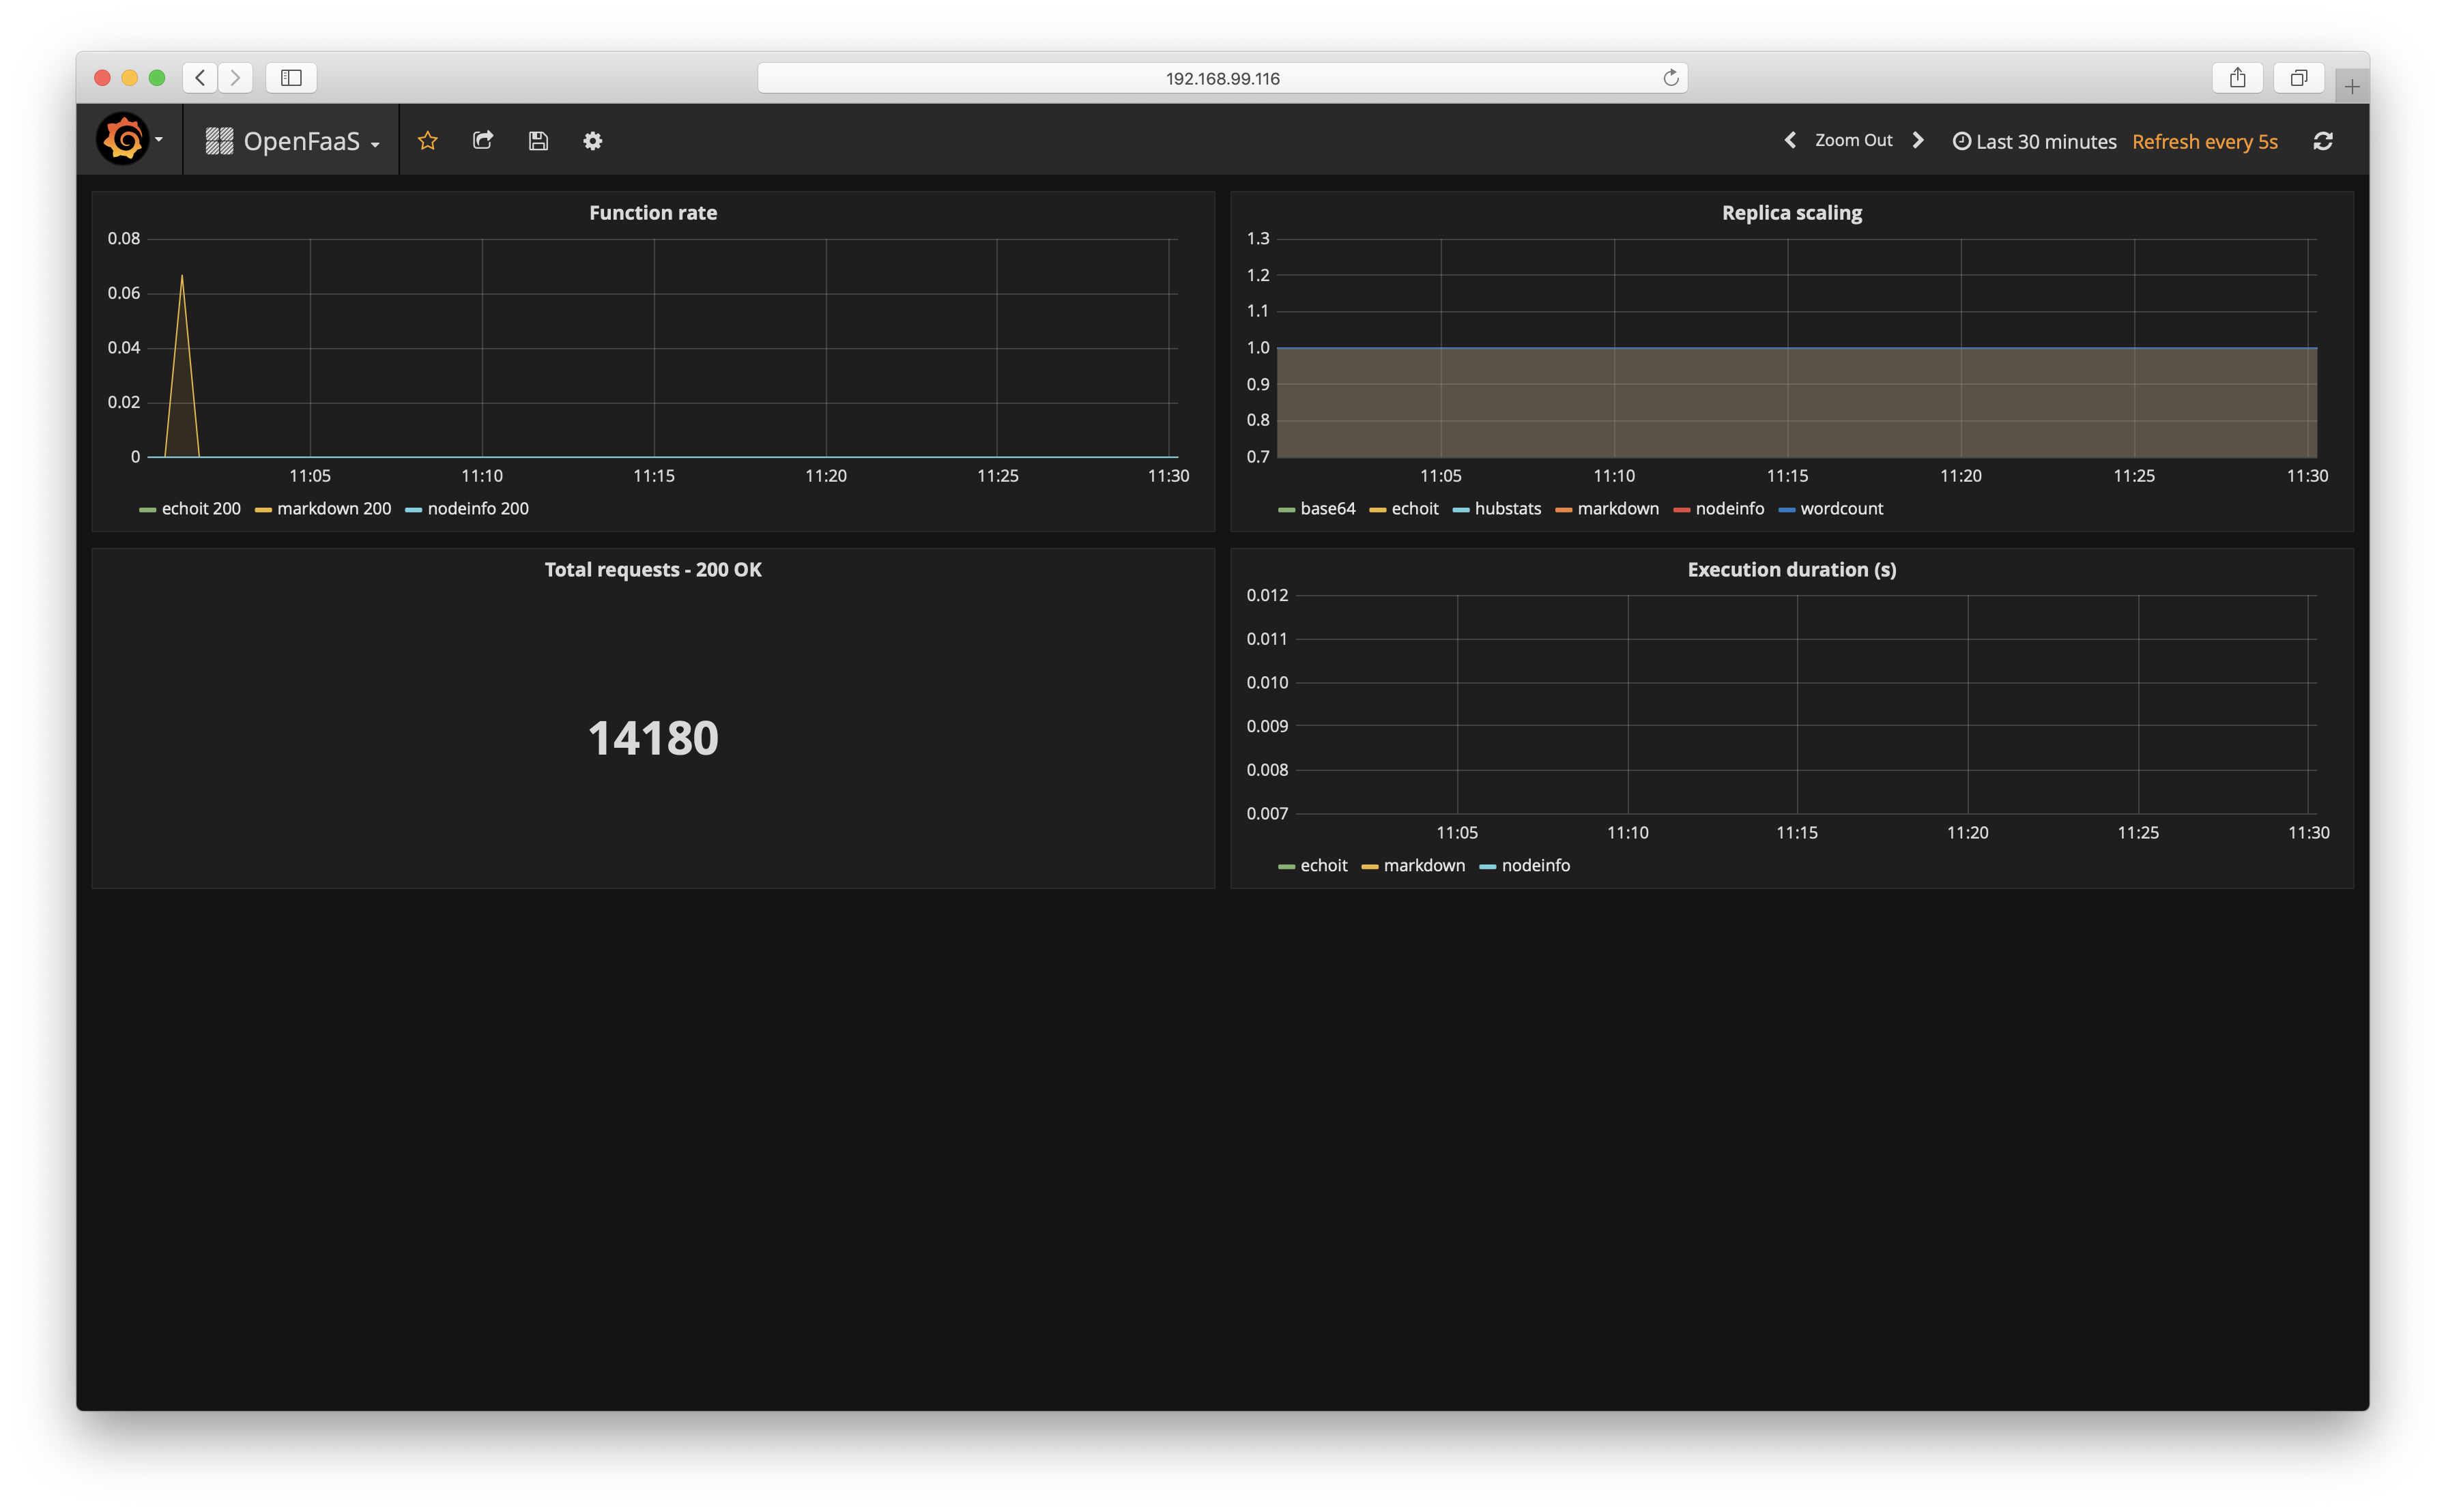
\includegraphics[width=1\textwidth]{img/grafana-dashboard.png}
    \caption{Grafana dashboard}
    \label{fig:grafana-dashboard}  
\end{figure}

\subsection{Deployment demofunctie}
